% !TEX root = CSUR/main.tex

\section{Introduction}

Symbolic execution is a powerful static analysis technique introduced in the mid 70's to perform software testing (see, e.g.,~{\cite{K-CACM76} and~\cite{H-TSE77}})\mynote{IF: are references appropriate? Should we give more credits? It seems several groups introduced independently this technique}. The basic idea is to allow the program to take on ``symbolic'' -- instead of concrete -- input values. Program variables and control flow paths are associated with expressions and constraints in terms of those symbols during a symbolic execution of the program. Constraints are eventually solved via SMT (satisfiability modulo theories) solvers.

In this paper we survey the main aspects of symbolic execution and discuss its extensive use in the context of computer security\mynote{IF: want focus on security?} for finding software vulnerabilities by analyzing programs at the level of either source or binary code.
We start with a simple example that will introduce many of the fundamental issues discussed in remainder of the article.

\subsection{A warm up example}

Consider the C function shown in Figure~\ref{fig:example-1}: its most critical operation is the division performed at line 10. Albeit the code is relatively simple, each of the {\tt int} input values {\tt a}, {\tt b}, and {\tt c} can be assigned with $2^{32}$ distinct values, though only values leading to $x + y + z - 3 = 0$ would make the code crash. Hence, while techniques such as random testing could generate bottomless input tests for this function, it is unlikely that those inputs which make the code crash would be randomly picked up\mynote{Fuzzing?}. 
Symbolic execution overcomes these limitations by evaluating a piece of code using {\em symbols}, instead of concrete values, for its inputs. This makes it possible to reason on {\em classes of input values}, instead of single input instances. 

\begin{figure}[t]
\begin{lstlisting}[basicstyle=\ttfamily\small]
              1.  int foobar(int a, int b, int c) {
              2.    int x = 0, y = 0, z = 0;
              3.    if (a != 0)
              4.      x = -2;
              5.    if (b < 5) {
              6.      z = 2;
              7.      if (a == 0 && c != 0)
              8.        y = 1;
              9.    }
             10.    return a / (x + y + z - 3);
             11.  }
\end{lstlisting}
\caption{Example: a very simple C function}
\label{fig:example-1}
\end{figure}

In more details, every global or local variable is associated with a symbol $\alpha_i$.  At any point of the execution, the symbolic engine maintains:

\begin{itemize}
  \item  an execution state $(stmt,~pc)$ where:
\begin{itemize}
  \item $stmt$ is the statement to evaluate. For the time being we assume that $stmt$ can be an assignment, a conditional branch or a jump (a discussion of more complex constructs for iteration and function calls will be provided in Section~\ref{example-discussion});
  \item $pc$ is a collection of path\mynote{IF: my feeling is that pc does not denote a set. Better notation? Isn't pc a logical formula?} constraints, i.e., a set of assumptions made over the symbols $\alpha_i$ in order to reach $stmt$. Initially $pc$ is empty, and is thus trivially satisfied.
\end{itemize}
\item a {\em memory mapping} $M$ for storing constraints over different symbols. This is required since in general every memory location can be associated with a symbol\mynote{Rephrase}.
\end{itemize}

\noindent Depending on $stmt$, the symbolic engine modifies the state as follows:
\begin{itemize}
  \item $stmt$ is a constant assignment $\alpha_i = c$: when a constant value $c$ is assigned to a variable associated to the symbol $\alpha_i$, $pc$ is extended by adding a constraint on $\alpha_i$:\mynote{Redundant? IF: I would remove the constant assignment}
    \[ pc \gets pc \wedge \alpha_i = c\]

  \item $stmt$ is an assignment $\alpha_i = e$: when an expression $e$ is assigned to a symbol $\alpha_i$, $pc$ is extended by adding a constraint on $\alpha_i$:
    \[ pc \gets pc \wedge \alpha_i = e\]
  where $e$ can be any expression, involving unary or binary operators, over symbols and constants.

  \item $stmt $ is a conditional branch ${\tt if}~e~{\tt then}~s_{true}~{\tt else}~s_{false}$: $pc$ is evaluated. Two scenarios are possible:
    \begin{itemize}
      \item (non-forking) $e$ is evaluated as always true or false under the assumptions in $pc$: the proper branch is taken, and symbolic execution advances to $s_{true}$ or $s_{false}$ accordingly;
      \item (forking) $e$ cannot be evaluated without instantiating values for one or more symbols in it: the symbolic execution process is forked, creating two execution states:
        \[ (s_{true}, pc_{true}) \text{ where } pc_{true} = pc \wedge e \]
        \[ (s_{false}, pc_{false}) \text{ where } pc_{false} = pc \wedge \neg e \]
    \end{itemize}
    Symbolic execution proceeds on both states in parallel.

  \item $stmt $ is a jump {\tt goto} $s$: execution state is updated to advance symbolic execution to $s$. 
\end{itemize}





\subsection{Removed stuff}

\paragraph{Black-box approach versus white-box approach}

Discussion\mynote{IF: do we really need this?} of black-box approach and white-box approach. Symbolic execution is a white-box technique. Black-box approaches can be very fast but not always effective. White-box approaches can be very effective but are typically slower than black-box techniques. An in-depth discussion of this aspect will be done when we will discuss~\cite{DRILLER-NDSS16}.

\begin{figure}[H]
  \vspace{-3mm}
  \centering
  \begin{subfigure}{.5\textwidth}
    \centering
    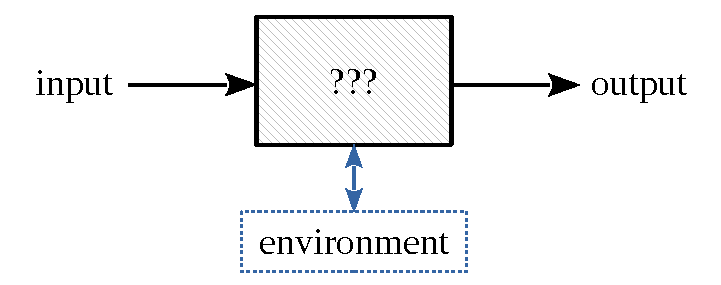
\includegraphics[width=0.9\linewidth]{images/blackbox} 
    \caption{Black-box approach}
    %\label{fig:sub1}
  \end{subfigure}%
  \begin{subfigure}{.5\textwidth}
    \centering
    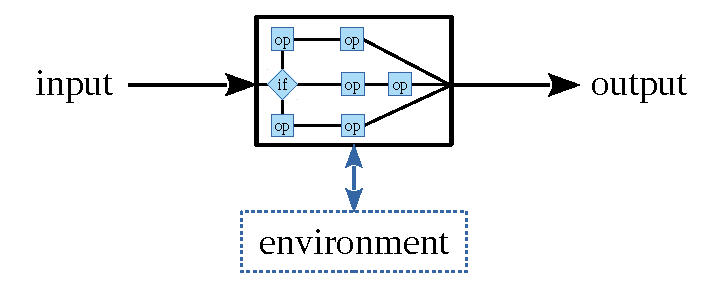
\includegraphics[width=0.9\linewidth]{images/whitebox} 
    \caption{White-box approach}
    %\label{fig:sub2}
  \end{subfigure}
  %\label{fig:example-symbolic-execution}
  \vspace{-3mm}
\end{figure}

\paragraph{Taken from old Overview}

Symbolic execution has been originally introduced in~\cite{K-CACM76} and~\cite{H-TSE77}. A good introduction to symbolic execution is presented in~\cite{KLEE-OSDI08}.\mynote{Extend this paragraph}
%(while~\cite{EXE-CCS06} is a previous effort of the same authors).
\cite{SAGE-NDSS08} is one successful story of symbolic execution. \cite{SAB-SP10} presents a neat formalization of symbolic execution and of taint analysis as well.

